\documentclass[12pt]{article}
\usepackage[a4paper, margin=2.5cm]{geometry}
\usepackage[hidelinks]{hyperref}
\usepackage[utf8]{inputenc}
\usepackage[T1]{fontenc}
\usepackage[polish]{babel}
\usepackage{listings}
\usepackage{booktabs}
\usepackage{float}
\usepackage{graphicx}
\graphicspath{{./}}
\lstset{language=Python,breaklines=true,breakatwhitespace=true,basicstyle=\ttfamily\small,captionpos=b}

\title{\textbf{Systemy złożone i analiza danych} \\ \textbf{Sprawozdanie z 7. zadania}}
\author{\textbf{Mieszko Czubiński} \\ Nr albumu: \textbf{284047}}
\date{\today}

\begin{document}

\maketitle

\section{Projekt algorytmu}

\subsection{Algorytm}

Celem algorytmu jest \textbf{wykrywanie anomali} krawędzi w sieci społecznej. Anomalią nazywamy krawędź, która łączy bezpośrednio dwie peryferyjne postacie, mimo że bez tej krawędzi byłyby one od siebie oddalone o wiele kroków (czyli normalnie komunikowałyby się przez łańcuch hubów). Jednym z zastosowań jest wykrywanie krawędzi, które prawdopodobnie nie powinny były powstać. Wskazane krawędzie można usunąć z sieci albo potraktować jako sygnał wymagający bliższej analizy.

Punktem wyjścia było proste pytanie: na ile dana krawędź jest ,,skrótem''? Aby to zmierzyć, można porównać bezpośrednie połączenie z najlepszą alternatywą -- usunąć krawędź $(u,v)$ i sprawdzić, ile kroków trzeba pokonać, żeby dotrzeć z $u$ do $v$ inną drogą. W sieci społecznej połączonej hubami takie ,,skróty'' mają również krawędzie pomostowe między samymi hubami, co jest natulane. Jako, że komunikacja zwykle przebiega przez huby, anomalią jest dopiero bezpośrednie połączenie dwóch peryferyjnych wierzchołków. Dlatego do długości objazdu dołączono peryferyjność obu końców (oparta na hubowości). W skrócie: zamiast ,,jak długi objazd'' sprawdzamy ,,jak długi objazd między peryferiami''.

\subsection{Schemat działania}

Algorytm dla każdej krawędzi $(u,v)$ liczy wynik $\mathrm{score}(u,v)$ łączący długość objazdu z peryferyjnością obu końców:

\begin{enumerate}
    \item \textbf{Hubowość.} Dla każdego wierzchołka wyznaczamy $\mathrm{hubness}(n) \in [0,1]$ jako rangę jego stopnia, znormalizowaną do przedziału $[0,1]$ (najsłabszy wierzchołek $0$, najsilniejszy $1$).
    \item \textbf{Objazd.} Krawędź $(u,v)$ jest tymczasowo usuwana, a następnie liczona jest długość najkrótszej ścieżki $u \rightarrow v$ w pozostałym grafie ($\mathrm{hops}$). Jeśli nie ma alternatywnej trasy -- krawędź jest pomijana.
    \item \textbf{Peryferyjność.} $\mathrm{periph}(u,v) = (1 - \mathrm{hubness}(u)) \cdot (1 - \mathrm{hubness}(v))$. Wartość bliska $1$ oznacza dwa peryferyjne końce; bliska $0$ -- że któryś z końców jest hubem.
    \item \textbf{Wynik.} $\mathrm{score}(u,v) = \mathrm{hops} \cdot \mathrm{periph}$. Wysoki, gdy długi objazd oraz peryferyjne końce.
    \item \textbf{Próg.} Krawędzie sortujemy malejąco po wyniku; jako anomalie oznaczamy górny odsetek.
\end{enumerate}

\subsection{Inne rozwiązania}

Problem wskazywania ,,nietypowych'' krawędzi można zrealizować również kilkoma prostymi, powszechnie znanymi metodami:

\begin{itemize}
    \item \textbf{Mosty (bridges).} Krawędź, której usunięcie rozspaja graf na dwie części (funkcja \texttt{nx.bridges}). Wykrywa jedynie skrajny przypadek -- krawędzie, które nie mają żadnej alternatywnej trasy.
    \item \textbf{Odwrócona predykcja połączeń.} Klasyczne miary podobieństwa wierzchołków (Common Neighbors, Jaccard) szacują, jak prawdopodobna jest krawędź. Istniejąca krawędź o bardzo niskim wyniku jest nieoczekiwana.
\end{itemize}

\section{Implementacja}

\subsection{Technologie}

Algorytm stworzono w języku \texttt{Python}, wykorzystując biblioteki \texttt{NetworkX} oraz \texttt{NumPy}. Do wyświetlenia danych użyto biblioteki \texttt{Seaborn}.

\subsection{Implementacja}

Rdzeń algorytmu przedstawia listing~\ref{lst:algorithm}. Funkcja \texttt{compute\_hubness} wyznacza hubowość, \texttt{detour\_hops} liczy długość objazdu po usunięciu krawędzi, a \texttt{detect\_anomalies} składa wyniki, sortuje krawędzie i oznacza górny odsetek jako anomalie.

\begin{lstlisting}[caption={Rdzeń algorytmu wykrywania anomalnych krawędzi.},label={lst:algorithm}]
def compute_hubness(G):
    deg = dict(G.degree())
    order = sorted(deg, key=lambda n: deg[n])
    n = len(order)
    if n <= 1:
        return {node: 1.0 for node in order}
    return {node: rank / (n - 1) for rank, node in enumerate(order)}


def detour_hops(G, u, v):
    data = dict(G[u][v])
    G.remove_edge(u, v)
    try:
        d = nx.shortest_path_length(G, u, v)
    except nx.NetworkXNoPath:
        d = None
    G.add_edge(u, v, **data)
    return d


def detect_anomalies(G, top_frac=TOP_FRAC):
    hub = compute_hubness(G)
    rows = []
    for u, v in list(G.edges()):
        d = detour_hops(G, u, v)
        if d is None:
            continue
        periph = (1.0 - hub[u]) * (1.0 - hub[v])
        rows.append({'u': u, 'v': v, 'hub_u': hub[u], 'hub_v': hub[v], 'hops': d, 'periph': periph, 'score': d * periph})

    rows.sort(key=lambda r: r['score'], reverse=True)
    n_anom = round(top_frac * len(rows))
    thr = rows[n_anom - 1]['score'] if 0 < n_anom <= len(rows) else float('inf')
    for i, r in enumerate(rows):
        r['significant'] = i < n_anom

    return {'hubness': hub, 'edges': rows, 'top_frac': top_frac, 'threshold': thr}
\end{lstlisting}

\section{Testy i wyniki}

Algorytm uruchomiono na sieci rzeczywistej (graf relacji postaci sagi o wiedźminie, zbudowany ze współwystąpień w tekście) oraz na sieci losowej Barabási--Albert (BA) o tej samej liczbie wierzchołków i zbliżonej liczbie krawędzi. Model BA wybrano jako odniesienie, ponieważ jest najbliższy strukturalnie sieci społecznej.

Tabela~\ref{tab:hubs_org} przedstawia dziesięć wierzchołków o najwyższej hubowości w sieci rzeczywistej. Tabela~\ref{tab:anomalies_org} zawiera dziesięć krawędzi o najwyższym wyniku $\mathrm{score}$; widać, że oba końce każdej z nich mają niską hubowość (peryferia), a długość objazdu wynosi 4--6 kroków.

\begin{table}[H]
    \centering
    \begin{tabular}{lr}
        \toprule
        Postać & hubness \\
        \midrule
        Geralt of Rivia   & 1.0000 \\
        Ciri              & 0.9979 \\
        Yennefer          & 0.9958 \\
        Emhyr var Emreis  & 0.9937 \\
        Falka             & 0.9916 \\
        Philippa Eilhart  & 0.9895 \\
        Vilgefortz        & 0.9874 \\
        Triss Merigold    & 0.9853 \\
        Milva             & 0.9832 \\
        Jarre             & 0.9811 \\
        \bottomrule
    \end{tabular}
    \caption{Dziesięć wierzchołków o najwyższej hubowości w sieci rzeczywistej.}
    \label{tab:hubs_org}
\end{table}

\begin{table}[H]
    \centering
    \footnotesize
    \begin{tabular}{llrrrrr}
        \toprule
        Postać 1 & Postać 2 & $\mathrm{hubness}_u$ & $\mathrm{hubness}_v$ & objazd & preferencyjność & score \\
        \midrule
        Ilona Laux-Antille  & Yiolenta Suarez         & 0.273 & 0.275 & 6 & 0.528 & 3.166 \\
        Ilona Laux-Antille  & Leticia Charbonneau     & 0.273 & 0.277 & 6 & 0.526 & 3.157 \\
        Leticia Charbonneau & Jada Glevissig          & 0.277 & 0.279 & 6 & 0.522 & 3.130 \\
        Aurora Henson       & Herbert Stammelford     & 0.254 & 0.256 & 5 & 0.555 & 2.777 \\
        Aurora Henson       & Ivo Richert             & 0.254 & 0.258 & 5 & 0.554 & 2.769 \\
        Yanna of Murivel    & Klara Larissa de Winter & 0.262 & 0.264 & 5 & 0.543 & 2.715 \\
        Orestes Kopps       & Istvan Igalffy          & 0.323 & 0.367 & 6 & 0.429 & 2.572 \\
        Cairbre aep Diared  & Orestes Kopps           & 0.463 & 0.323 & 6 & 0.363 & 2.181 \\
        Marquard            & Rejean                  & 0.268 & 0.270 & 4 & 0.534 & 2.135 \\
        Vascoigne           & Istvan Igalffy          & 0.468 & 0.367 & 6 & 0.337 & 2.023 \\
        \bottomrule
    \end{tabular}
    \caption{Dziesięć krawędzi o najwyższym wyniku w sieci rzeczywistej.}
    \label{tab:anomalies_org}
\end{table}

Natomiast Tabela~\ref{tab:hubs_ba} przedstawia wierzchołki o najwyższej hubowości w sieci BA. A Tabela~\ref{tab:anomalies_ba} zawiera dziesięć krawędzi o najwyższym wyniku $\mathrm{score}$.

\begin{table}[H]
    \centering
    \begin{tabular}{lr}
        \toprule
        Wierzchołek & hubness \\
        \midrule
        4  & 1.0000 \\
        0  & 0.9979 \\
        11 & 0.9958 \\
        6  & 0.9937 \\
        10 & 0.9916 \\
        7  & 0.9895 \\
        13 & 0.9874 \\
        9  & 0.9853 \\
        5  & 0.9832 \\
        16 & 0.9811 \\
        \bottomrule
    \end{tabular}
    \caption{Dziesięć wierzchołków o najwyższej hubowości w sieci BA.}
    \label{tab:hubs_ba}
\end{table}

\begin{table}[H]
    \centering
    \footnotesize
    \begin{tabular}{llrrrrr}
        \toprule
        Wierzchołek 1 & Wierzchołek 2 & $\mathrm{hubness}_u$ & $\mathrm{hubness}_v$ & objazd & preferencyjność & score \\
        \midrule
        30  & 213 & 0.373 & 0.034 & 4 & 0.606 & 2.423 \\
        135 & 198 & 0.403 & 0.023 & 4 & 0.584 & 2.335 \\
        100 & 265 & 0.388 & 0.073 & 4 & 0.567 & 2.269 \\
        115 & 269 & 0.396 & 0.078 & 4 & 0.557 & 2.228 \\
        176 & 219 & 0.426 & 0.038 & 4 & 0.553 & 2.211 \\
        191 & 390 & 0.438 & 0.218 & 5 & 0.439 & 2.197 \\
        175 & 416 & 0.423 & 0.258 & 5 & 0.428 & 2.139 \\
        197 & 253 & 0.444 & 0.061 & 4 & 0.522 & 2.087 \\
        202 & 429 & 0.449 & 0.279 & 5 & 0.398 & 1.988 \\
        155 & 341 & 0.415 & 0.153 & 4 & 0.495 & 1.982 \\
        \bottomrule
    \end{tabular}
    \caption{Dziesięć krawędzi o najwyższym wyniku w sieci BA.}
    \label{tab:anomalies_ba}
\end{table}

Rozkład wyników wszystkich krawędzi (posortowanych malejąco) wraz z progiem odcięcia przedstawiają rysunki~\ref{fig:scores-original} (sieć rzeczywista) i~\ref{fig:scores-ba} (sieć BA). Wykryte anomalie na tle całej sieci pokazują rysunki~\ref{fig:graph-original} i~\ref{fig:graph-ba}.

\begin{figure}[H]
    \centering
    
\includegraphics[width=0.85\textwidth]{figures/anomaly_scores_original.png}
    \caption{Sieć rzeczywista: wynik $\mathrm{score}$ krawędzi wg rangi oraz próg (górny $1\%$).}
    \label{fig:scores-original}
\end{figure}

\begin{figure}[H]
    \centering
    
\includegraphics[width=0.85\textwidth]{figures/anomaly_scores_ba.png}
    \caption{Sieć Barabásiego--Alberta: wynik $\mathrm{score}$ krawędzi wg rangi oraz próg (górny $1\%$).}
    \label{fig:scores-ba}
\end{figure}

\begin{figure}[H]
    \centering
    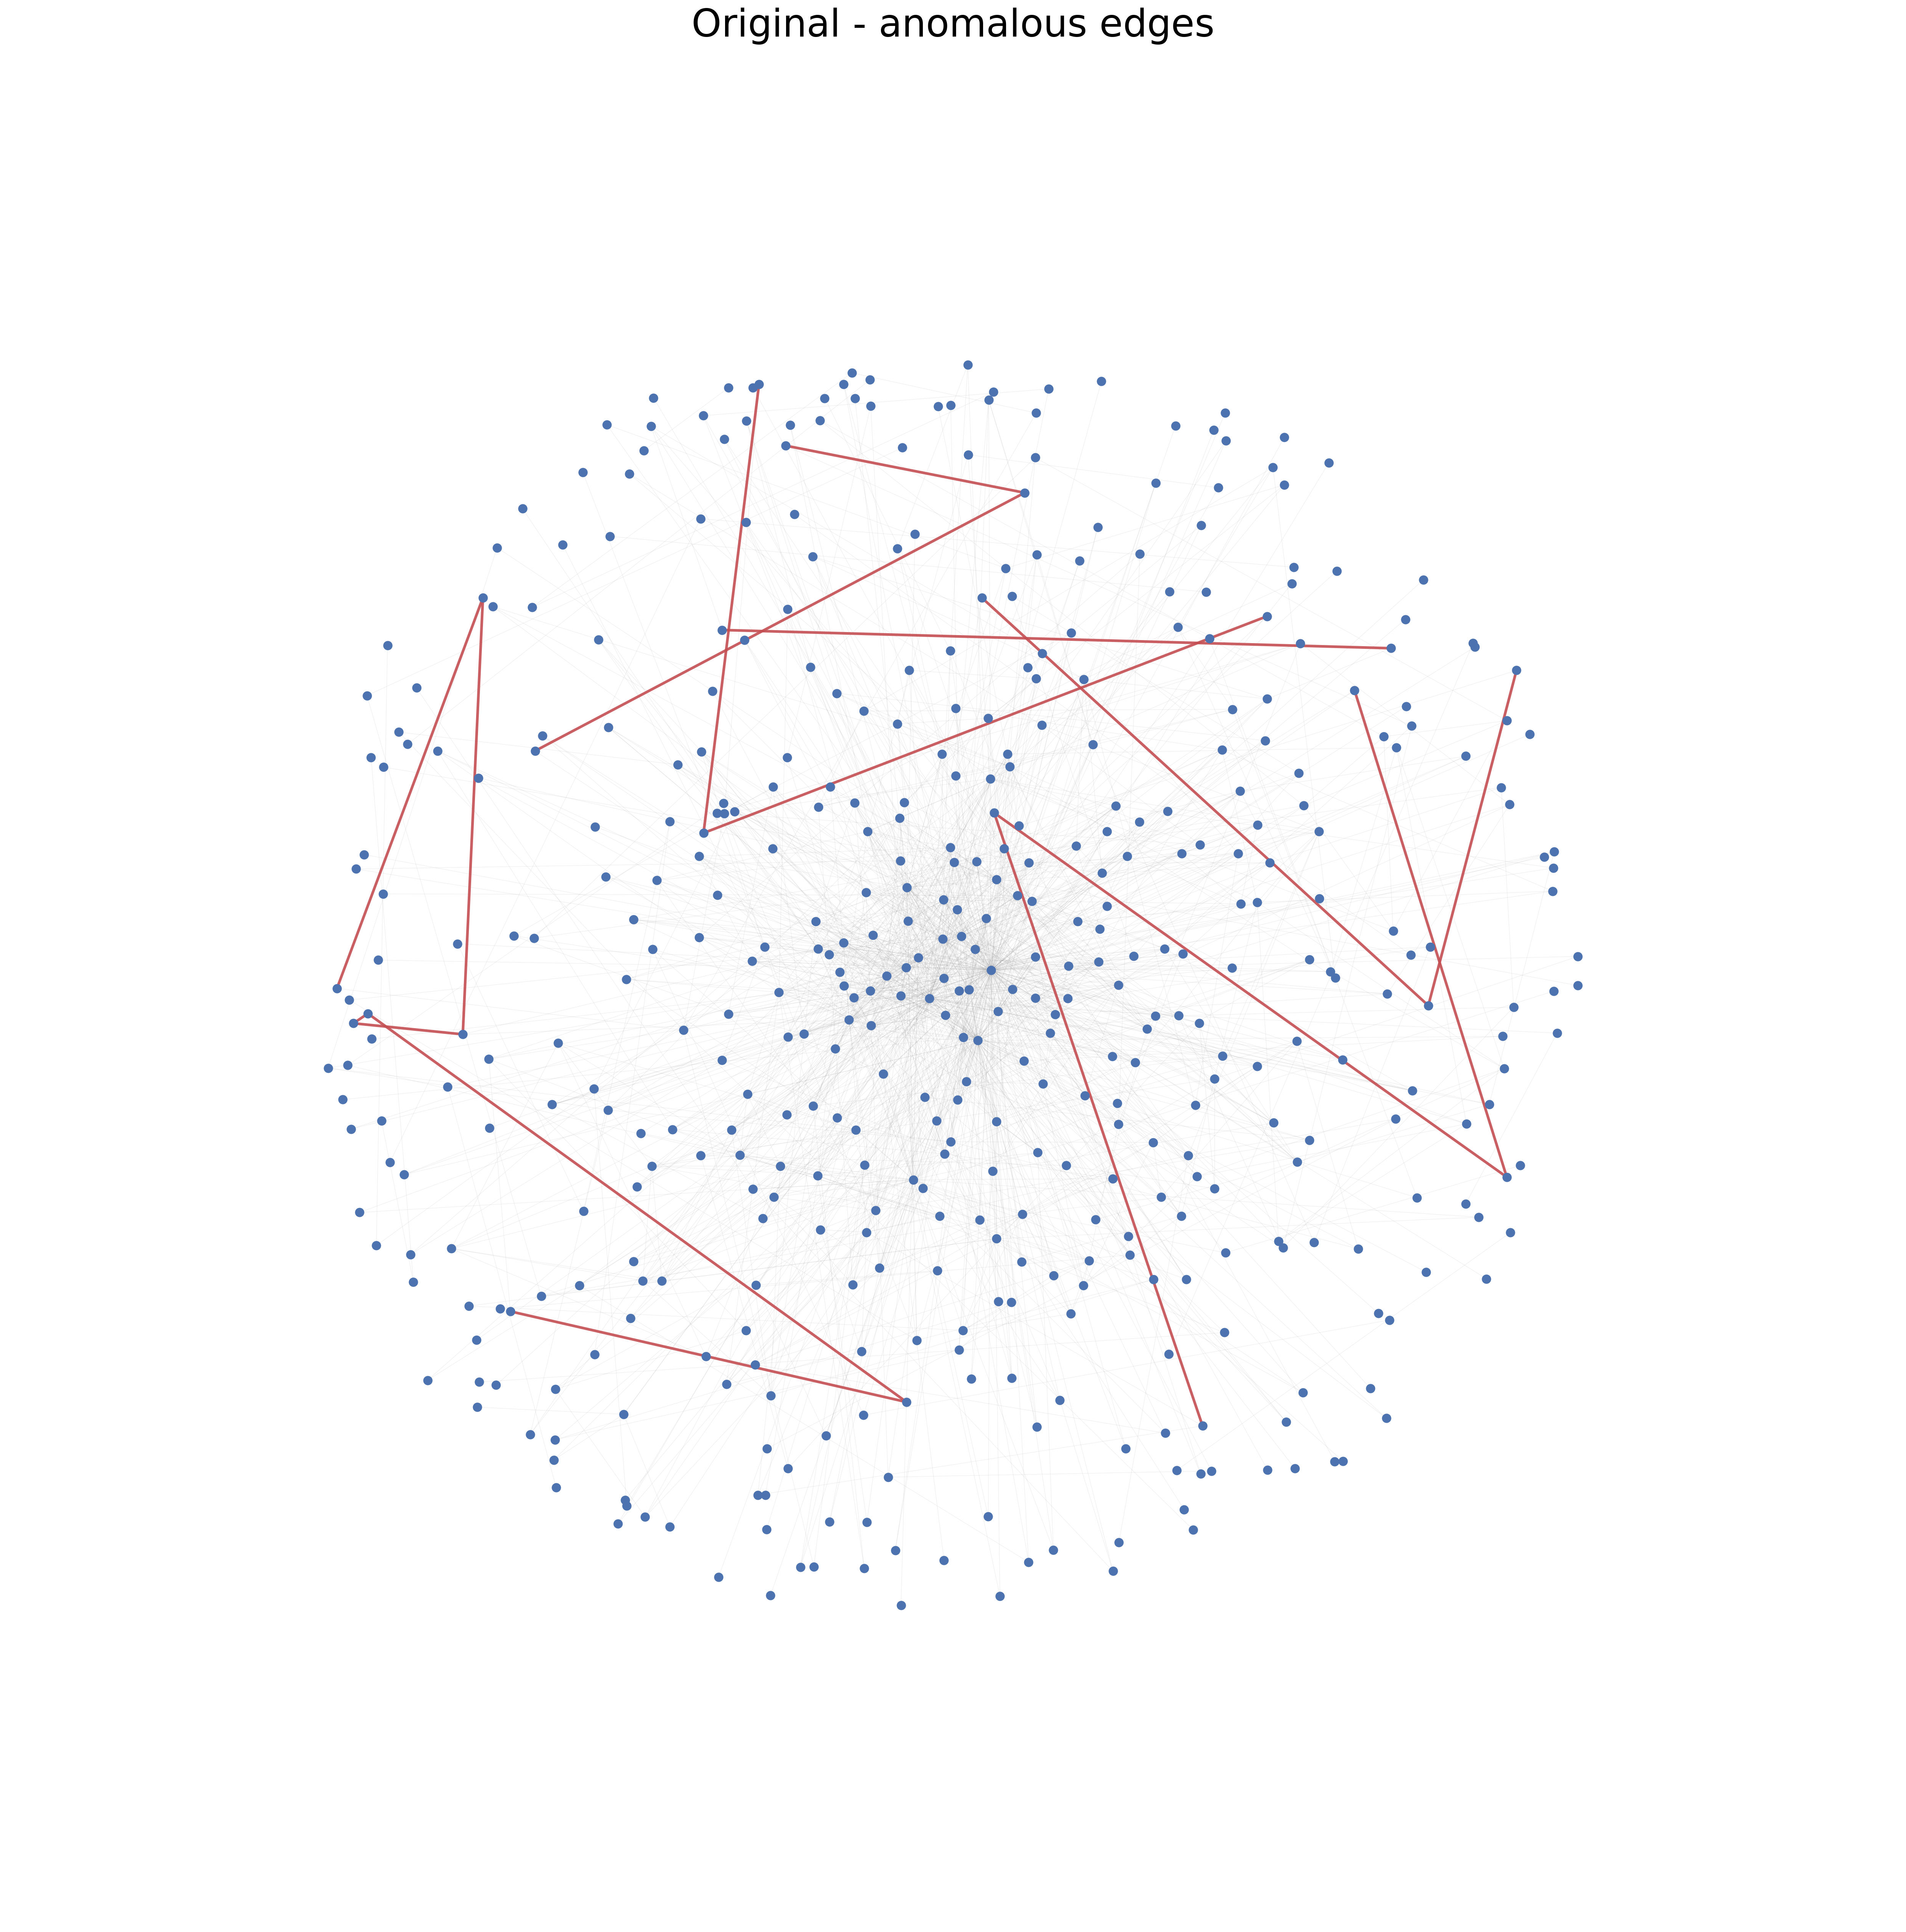
\includegraphics[width=0.7\textwidth]{figures/graph_anomalies_original.png}
    \caption{Sieć rzeczywista z zaznaczonymi anomaliami (kolor czerwony).}
    \label{fig:graph-original}
\end{figure}

\begin{figure}[H]
    \centering
    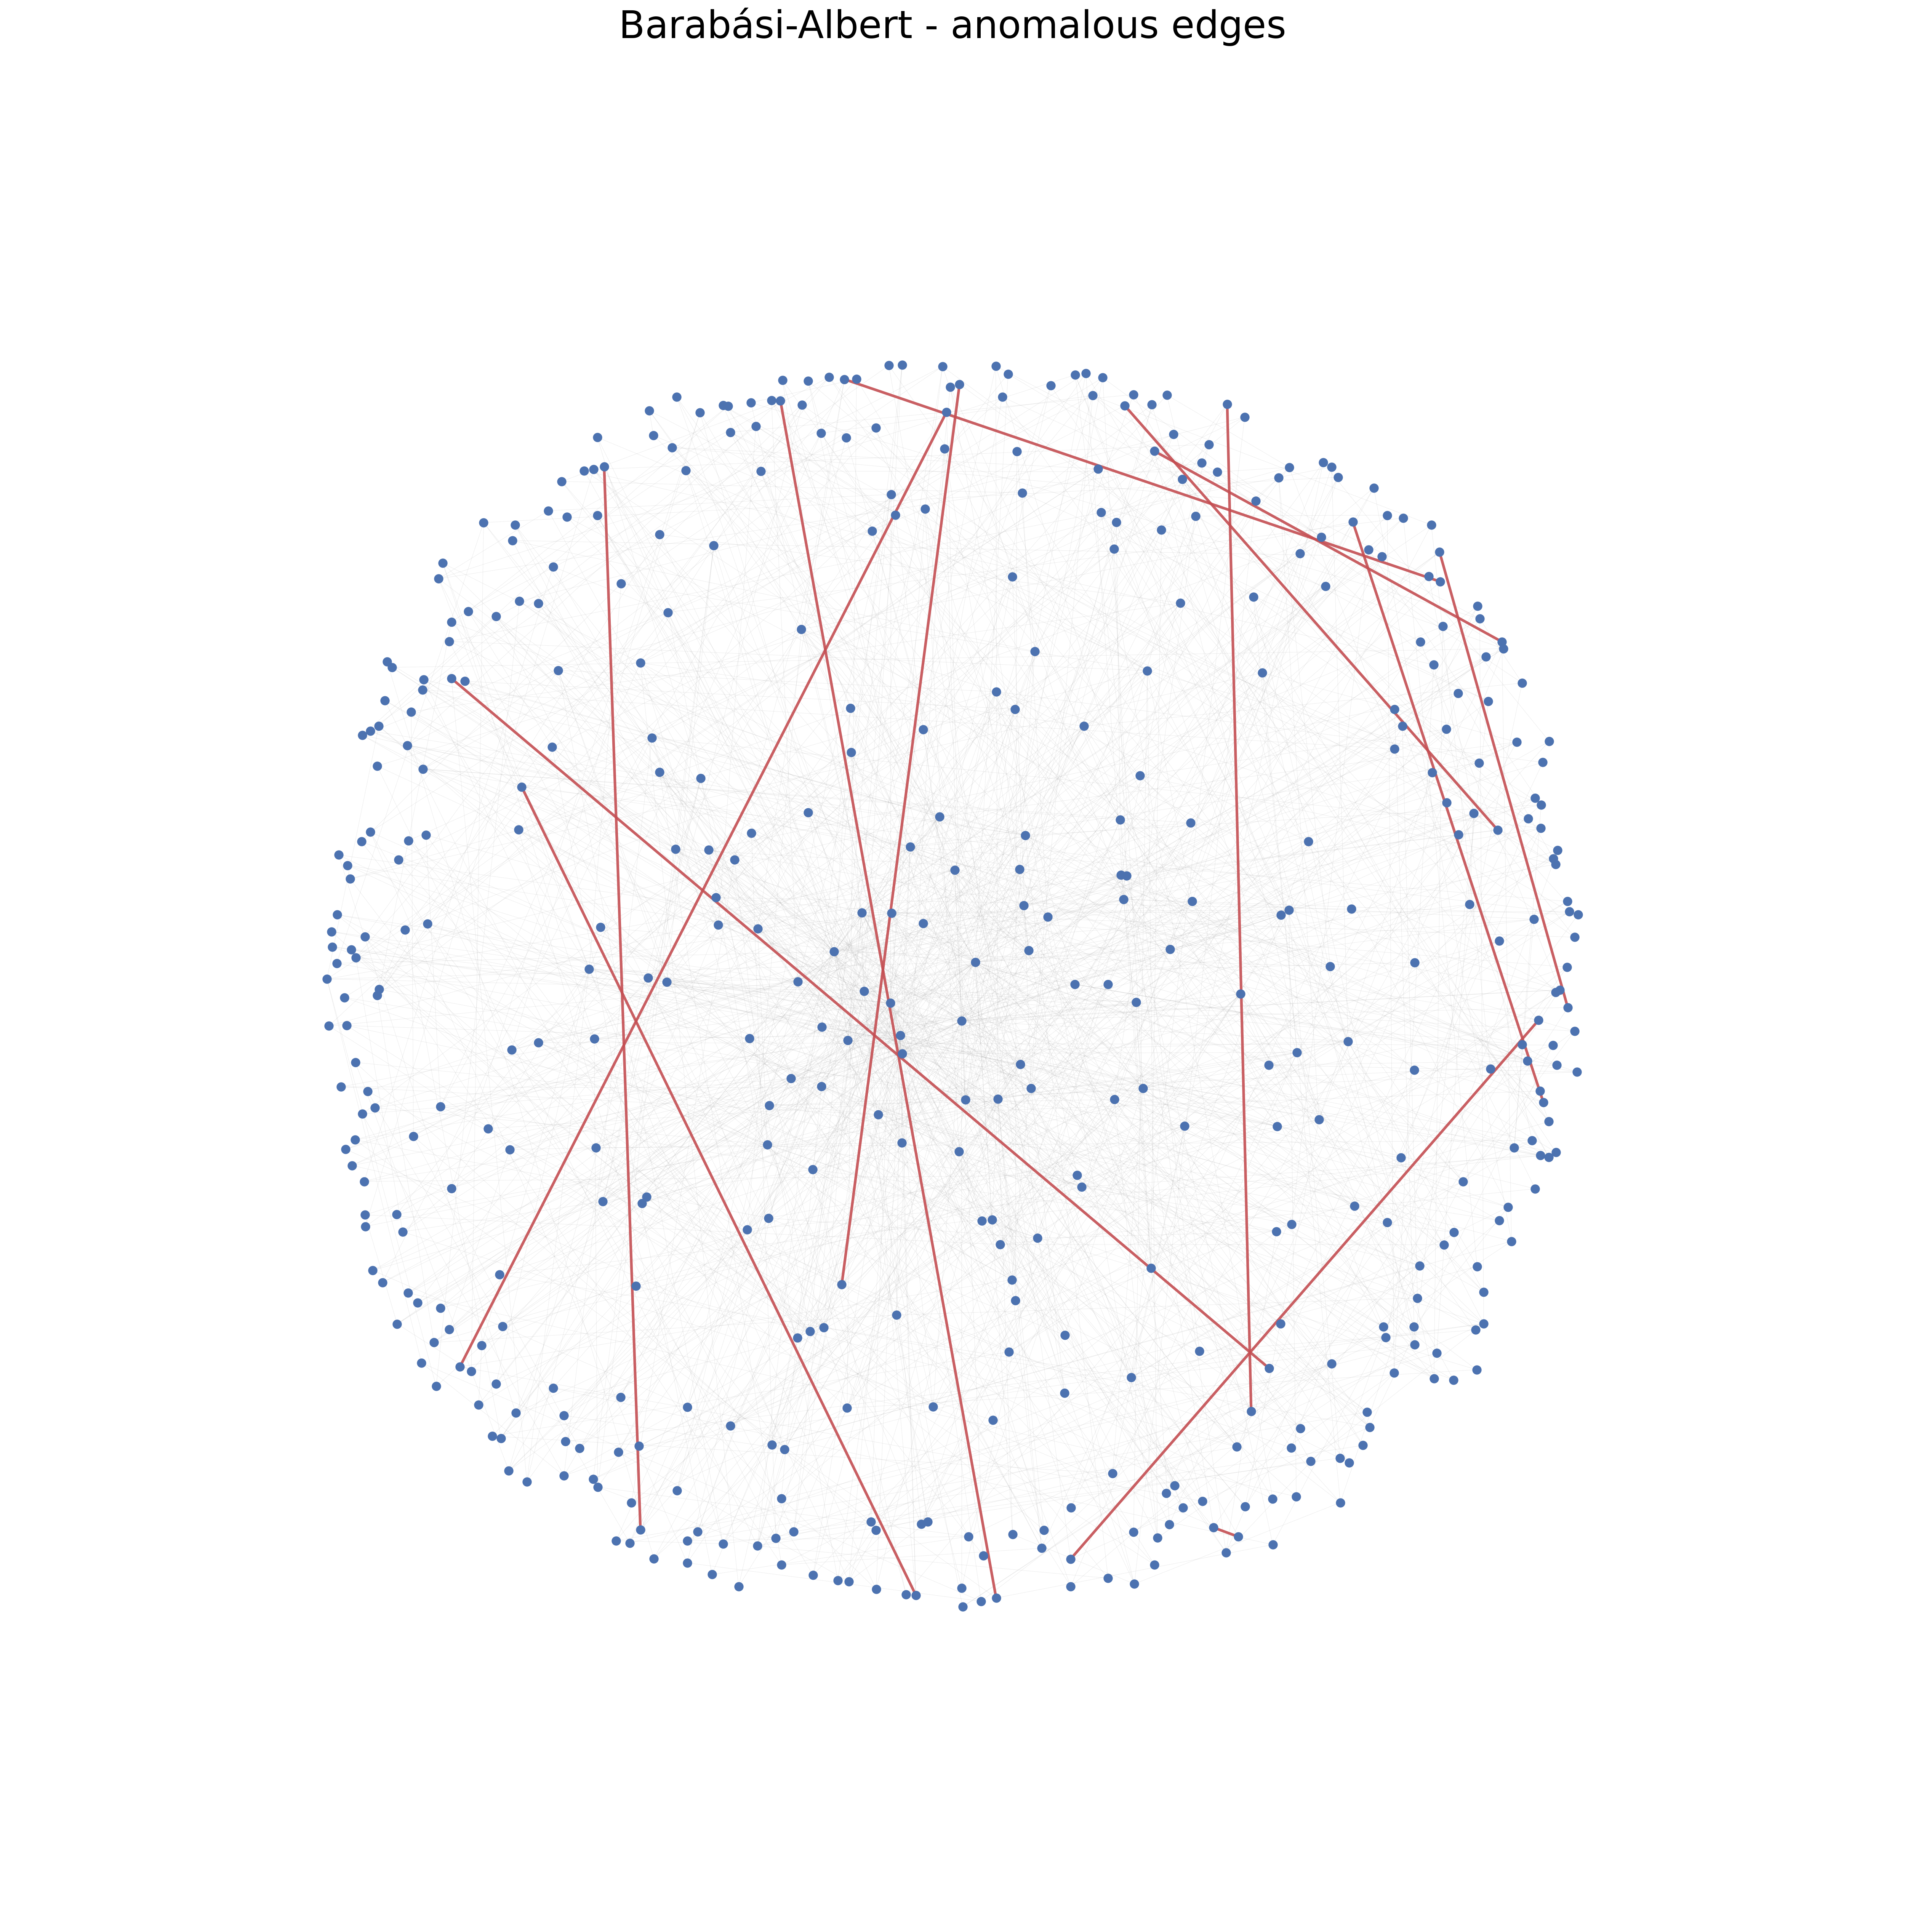
\includegraphics[width=0.7\textwidth]{figures/graph_anomalies_ba.png}
    \caption{Sieć Barabásiego--Alberta z zaznaczonymi anomaliami (kolor czerwony).}
    \label{fig:graph-ba}
\end{figure}

\section{Ocena algorytmu}

Porównanie obu sieci zestawia tabela~\ref{tab:comparison}. Przy tym samym odsetku odcięcia ($1\%$) sieć rzeczywista i sieć BA dają podobną liczbę anomalii, jednak \textbf{próg odcięcia w sieci BA jest wyraźnie wyższy} (1.927 wobec 1.555). Wynika to ze struktury: w sieci BA brak społeczności, więc peryferyjne wierzchołki są realnie dalej od siebie i większość krawędzi ma wyższy wynik. W sieci rzeczywistej społeczności trzymają peryferia blisko własnego huba, więc krawędzie ,,normalne'' mają niski wynik, a prawdziwe skróty wybijają się już przy niższym progu.

\begin{table}[H]
    \centering
    \begin{tabular}{lrr}
        \toprule
        Miara & Sieć rzeczywista & Sieć BA \\
        \midrule
        Wierzchołki                         & 478   & 478   \\
        Krawędzie ocenione                  & 1550  & 1425  \\
        Próg $\mathrm{score}$ (top $1\%$)   & 1.555 & 1.927 \\
        Liczba anomalii                     & 16    & 14    \\
        \bottomrule
    \end{tabular}
    \caption{Porównanie wyników działania algorytmu na sieci rzeczywistej i losowej (BA).}
    \label{tab:comparison}
\end{table}

\section{Wnioski}

Zaproponowany algorytm skutecznie wskazuje krawędzie będące dalekosiężnymi skrótami między peryferiami sieci, omijające huby. Jest prosty (kilka funkcji), w pełni topologiczny i samodostrajający się. Testy na sieci rzeczywistej i losowej pokazały, że wyniki są zgodne z intuicją.

\end{document}
